%!TEX root = Slic3r-Manual.tex

\subsection{Variable Layer Height} % (fold)
\label{sec:variable_layer_height}
\index{layer height}

Slic3r gives the ability to adjust the layer height between arbitrary positions along the Z axis.  That is, parts of the model could be printed with a coarse layer height, for example vertical subsections, and other parts could be printed with a finer layer height, for example sloping gradients where layering appears more pronounced.

The model in fig. \ref{fig:example_model} gives a rudimentary example of where variable layer heights could be used to improve print quality.  The walls of the structure need not be rendered in high definition for acceptable quality, however the sloping roof shows layer artifacts as the layer height of 0.4mm is too coarse, particularly for the very top, which is flattened.  This is shown in the G-Code rendering in fig \ref{fig:example_gcode_normal_layer_heights}.


\begin{figure}[H]
\centering
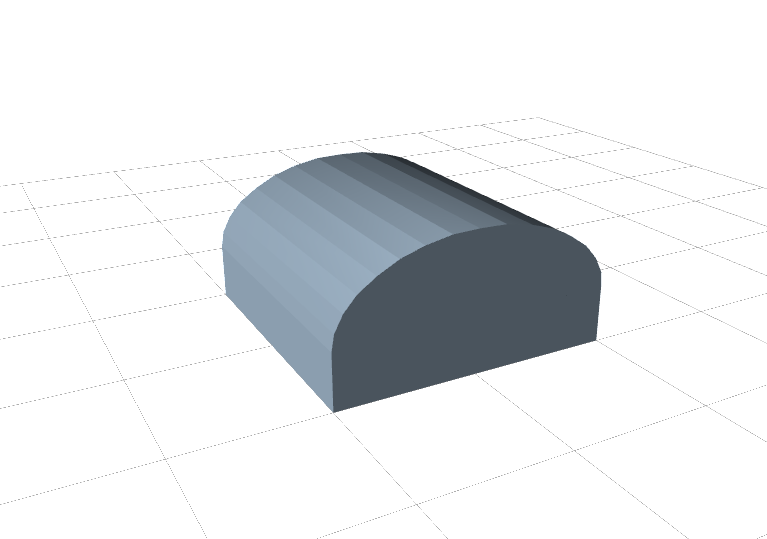
\includegraphics[keepaspectratio=true,width=0.75\textwidth]{expertmode/variable_layer_height/example_model.png}
\caption{Example model highlighting use case for variable layer heights.}
\label{fig:example_model}
\end{figure}

\begin{figure}[H]
\centering
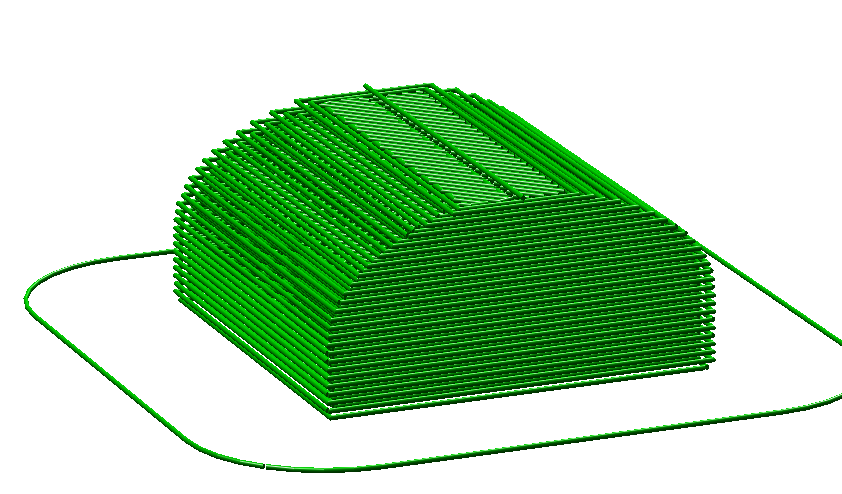
\includegraphics[keepaspectratio=true,width=0.75\textwidth]{expertmode/variable_layer_height/example_gcode_normal_layer_heights.png}
\caption{Example with normal layer height.}
\label{fig:example_gcode_normal_layer_heights}
\end{figure}

The variable layer height options are available by double clicking on a part name in the Plater window.  This will cause a pop-up window to be displayed which contains two tabs. The first gives some information about the model, as shown in fig. \ref{fig:variable_layer_height_options_tab_1}.

\begin{figure}[H]
\centering
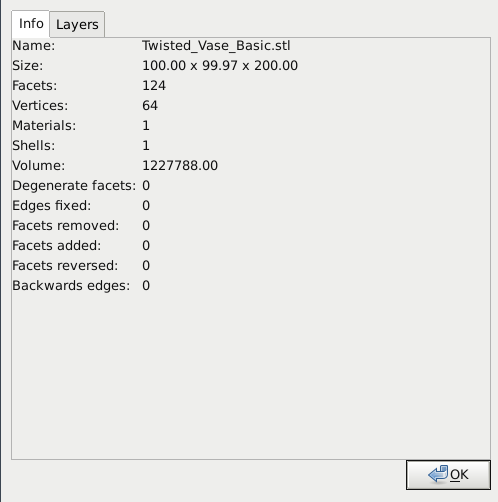
\includegraphics[keepaspectratio=true,width=0.75\textwidth]{expertmode/variable_layer_height/variable_layer_height_options_tab_1.png}
\caption{Variable layer height options - Info.}
\label{fig:variable_layer_height_options_tab_1}
\end{figure}

It is worth noting the height of the model, as this will be useful when calculating the maximum Z height.

The second tab (fig. \ref{fig:variable_layer_height_options_tab_2}) presents a table where each row defines a layer height for a particular range along the Z axis, given in millimeters.  In this example the walls of the model are printed at 0.4mm, the steeper parts of the roof are printed at 0.2mm, and the less steep at 0.15mm.  Note that each range divides exactly by the given layer height so there are no "gaps" between subsections.

\begin{figure}[H]
\centering
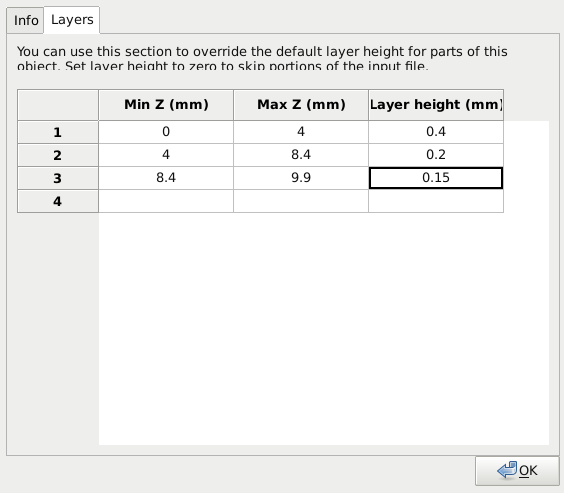
\includegraphics[keepaspectratio=true,width=0.75\textwidth]{expertmode/variable_layer_height/variable_layer_height_options_tab_2.png}
\caption{Variable layer height options - Layers.}
\label{fig:variable_layer_height_options_tab_2}
\end{figure}

The resulting G-Code (fig. \ref{fig:example_gcode_variable_layer_heights}) shows a higher definition which should result in a higher quality print.

\begin{figure}[H]
\centering
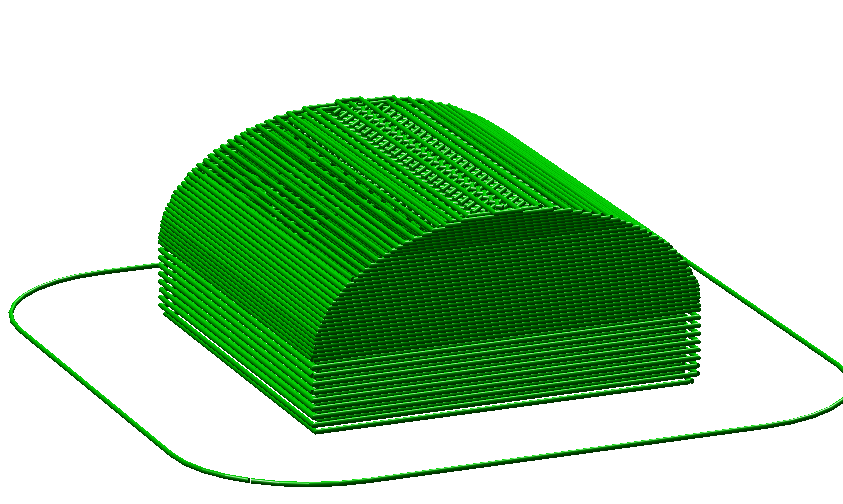
\includegraphics[keepaspectratio=true,width=0.75\textwidth]{expertmode/variable_layer_height/example_gcode_variable_layer_heights.png}
\caption{Example with variable layer height.}
\label{fig:example_gcode_variable_layer_heights}
\end{figure}

Fig. \ref{fig:example_print} shows the example model printed.  The print on the left has 0.4mm layer height throughout, whereas the print on the right has the variable layer height.

\begin{figure}[H]
\centering
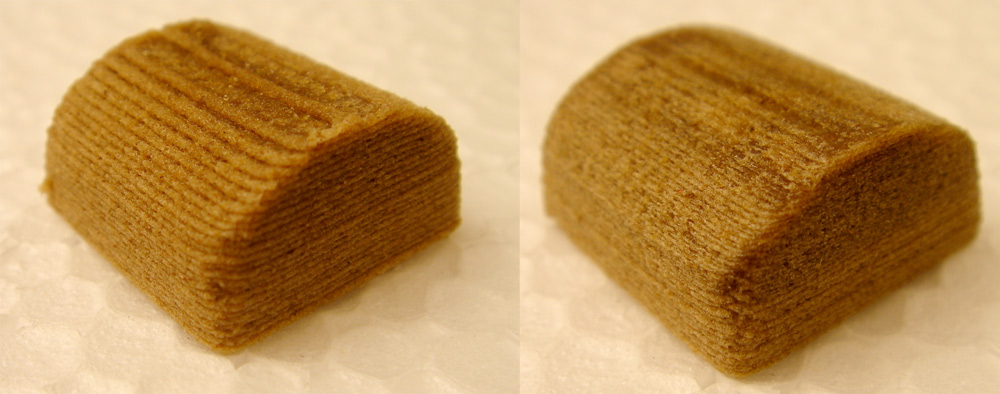
\includegraphics[keepaspectratio=true,width=1\textwidth]{expertmode/variable_layer_height/example_print.jpg}
\caption{Example print with variable layer height.}
\label{fig:example_print}
\end{figure}

An additional feature of the variable layers height option is that by entering a zero for a range that part of the model will not be printed.  Fig. \ref{fig:example_gcode_skipped_layers} shows the G-Code where layers between 0 and 4mm are skipped.  This is a useful way of dividing a tall model into multiple, shorter subsections which can be printed individually and assembled afterwards.
\begin{figure}[H]
\centering
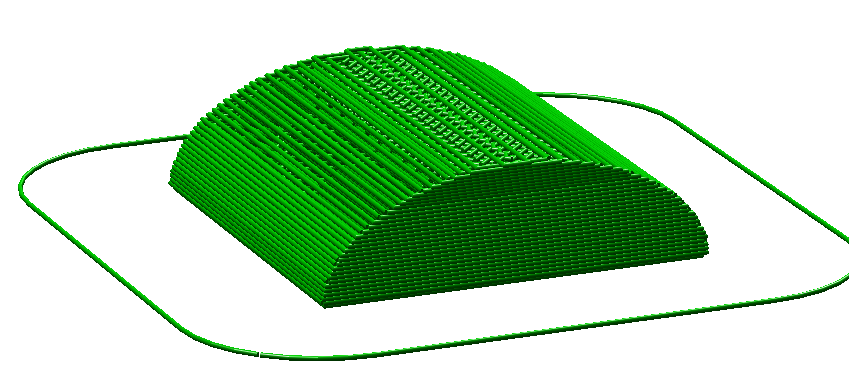
\includegraphics[keepaspectratio=true,width=0.75\textwidth]{expertmode/variable_layer_height/example_gcode_skipped_layers.png}
\caption{Example with skipped layers.}
\label{fig:example_gcode_skipped_layers}
\end{figure}

% subsection variable_layer_height (end)